\documentclass[12pt,a4paper]{tietreport}

% =========================================================
% TITLE PAGE
% =========================================================

\TitlePageHeader{


UCS503P - SOFTWARE ENGINEERNING PROJECT\\
}

\ProjectTitle{
BLURGUARD
}

\ProjectSubtitle{
AI-Based Real-Time Sensitive Data Detection and Masking
}

\TitlePageSubText{
Submitted by:
}

\AdvisorName{
Dr. Nisha Thakur
}

\TitlePageFooterText{
Mid-Semester Evaluation\\
Computer Science and Engineering Department\\
Thapar Institute of Engineering and Technology, Patiala
}

% =========================================================

\begin{document}

\maketiettitle

\tableofcontents

\clearpage

% =========================================================
% CHAPTER 1
% =========================================================

\chapter{Introduction}

\section{Background and Context}

Screenshots and screen-sharing sessions may contain sensitive information such as names, email addresses, phone numbers, identification numbers, passwords, API keys, and financial information.

Manual detection and masking of such information is time-consuming and may result in accidental data exposure.

\textbf{BlurGuard} is proposed as an AI-based privacy protection system that detects sensitive information from visual content and masks the detected regions before sharing.

The system combines OCR, image processing, pattern matching, computer vision, and risk assessment.

\subsection{Problem Statement}

The main problem is the accidental exposure of sensitive information through screenshots, application windows, documents, and screen-sharing sessions.

BlurGuard aims to automate this process by:

\begin{itemize}
    \item detecting sensitive information,
    \item identifying its location,
    \item assessing its risk, and
    \item masking the sensitive region.
\end{itemize}

\section{Project Objectives}

The main objectives are:

\begin{enumerate}
    \item Detect sensitive information from images and screenshots.
    \item Extract text using OCR.
    \item Identify structured information using pattern matching.
    \item Classify detected information according to risk.
    \item Mask sensitive regions automatically.
    \item Provide a user interface for monitoring privacy protection.
\end{enumerate}

% =========================================================
% CHAPTER 2
% =========================================================

\chapter{Methodology and Design}

\section{System Architecture}

BlurGuard follows a modular pipeline:

\begin{center}
\textbf{Capture}
$\rightarrow$
\textbf{Preprocess}
$\rightarrow$
\textbf{OCR}
$\rightarrow$
\textbf{Detect}
$\rightarrow$
\textbf{Risk Assessment}
$\rightarrow$
\textbf{Mask}
\end{center}

The major modules are:

\begin{itemize}
    \item Screen Capture
    \item Image Preprocessing
    \item OCR
    \item Sensitive Data Detection
    \item Risk Assessment
    \item Masking
    \item User Interface
\end{itemize}

\subsection{Technical Stack}

\begin{table}[H]
\centering
\caption{Technical Stack}

\begin{tabularx}{\textwidth}{lX}
\toprule
\textbf{Technology} & \textbf{Purpose}\\
\midrule
Python & Backend processing\\
OpenCV & Image processing\\
Tesseract OCR & Text extraction\\
FastAPI & Backend API\\
React & User interface\\
TypeScript & Frontend development\\
Vite & Development environment\\
Git/GitHub & Version control\\
\bottomrule
\end{tabularx}

\end{table}

\section{Implementation Details}

\subsection{Frontend Interface}

The frontend provides the main interface for accessing and monitoring BlurGuard.

\begin{figure}[H]
\centering
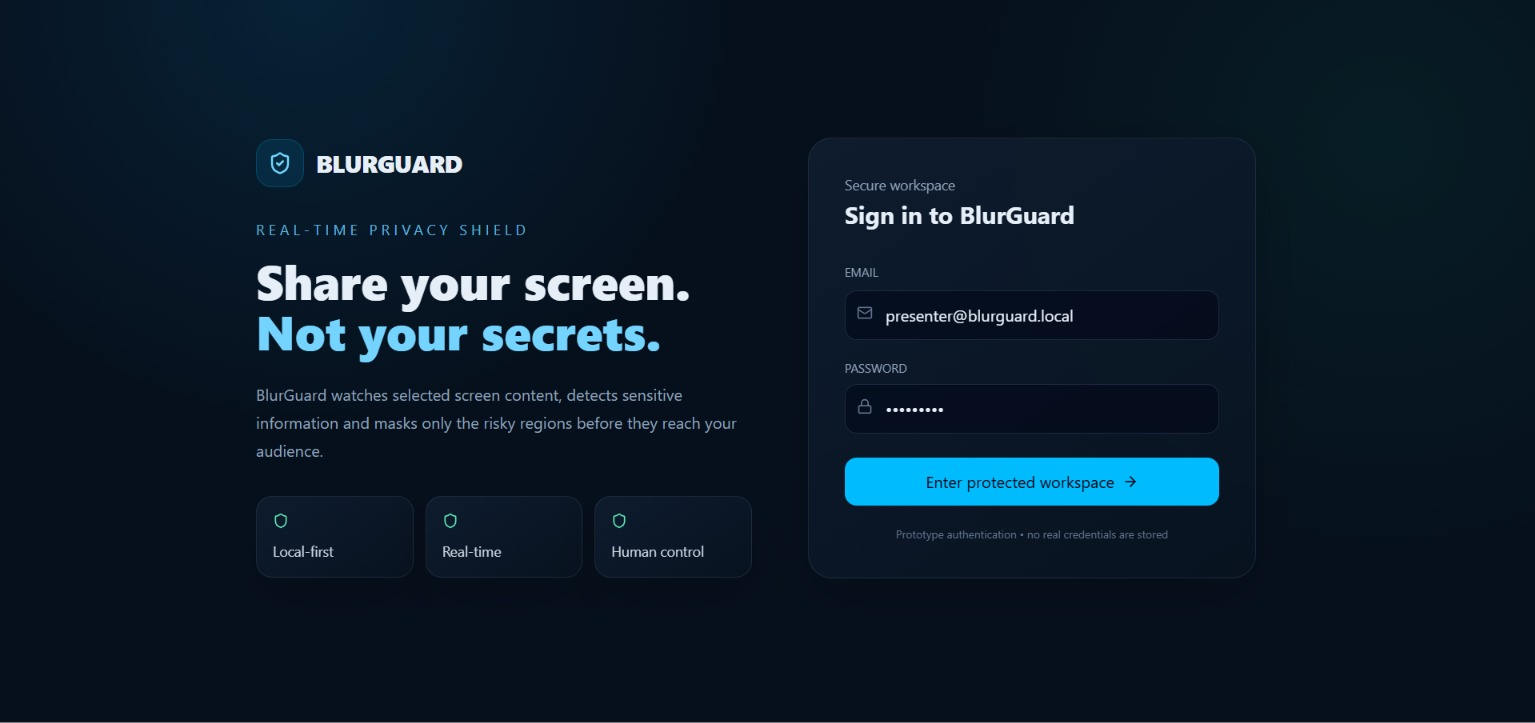
\includegraphics[width=0.88\textwidth]{login_screen.jpg}
\caption{BlurGuard Secure Workspace}
\end{figure}

\begin{figure}[H]
\centering
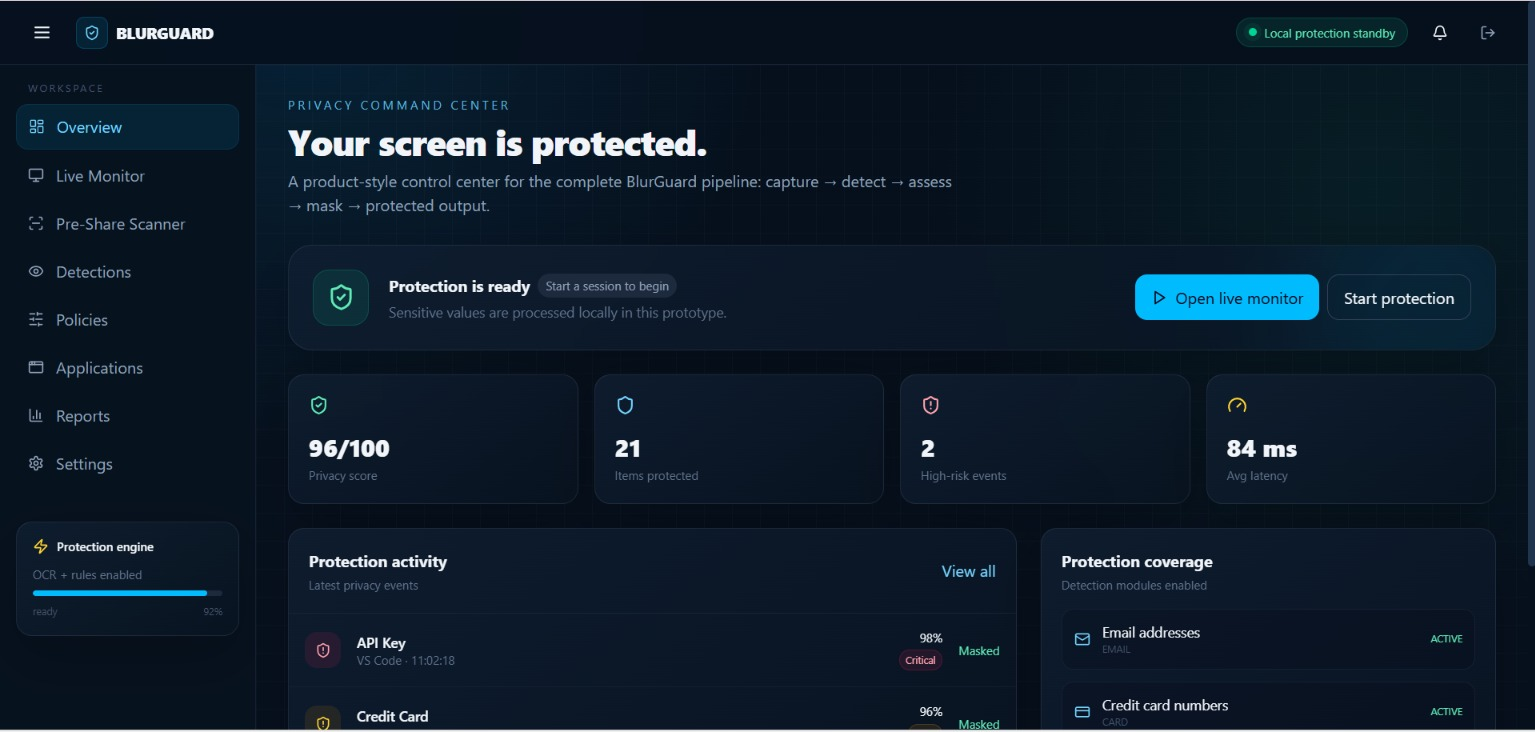
\includegraphics[width=0.92\textwidth]{dashboard.jpg}
\caption{BlurGuard Privacy Command Center}
\end{figure}

\begin{figure}[H]
\centering
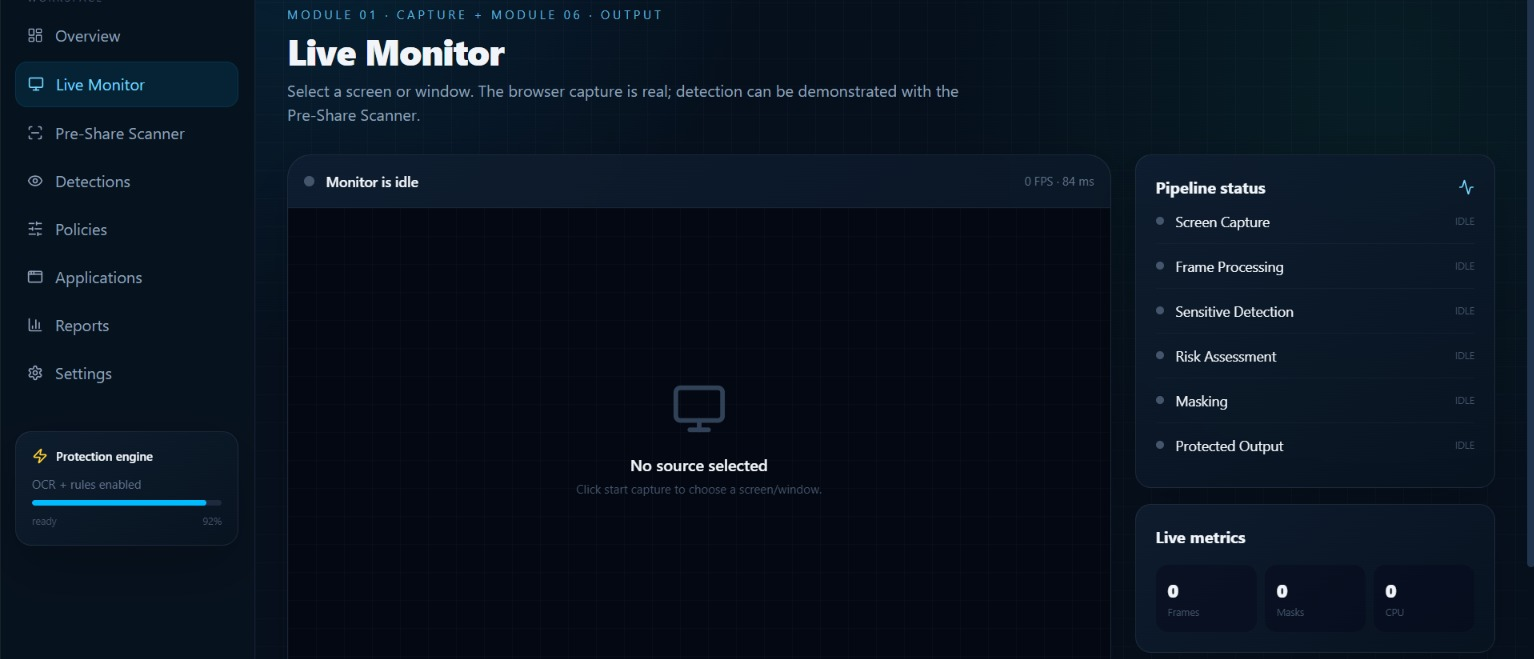
\includegraphics[width=0.92\textwidth]{live_monitor.jpg}
\caption{BlurGuard Live Monitoring Interface}
\end{figure}

\subsection{Detection and Masking}

The system uses OCR to extract visible text and pattern-based techniques to identify sensitive information.

Target categories include:

\begin{itemize}
    \item Personal information
    \item Email addresses
    \item Phone numbers
    \item Financial information
    \item Passwords and credentials
    \item API keys and access tokens
\end{itemize}

Detected information is assigned a risk level and protected using blur, pixelation, solid masking, or redaction.

\section{System Modeling and Project Diagrams}

\subsection{Activity Diagram}

The activity diagram represents the flow from screen monitoring to detection and masking.

\begin{figure}[H]
\centering
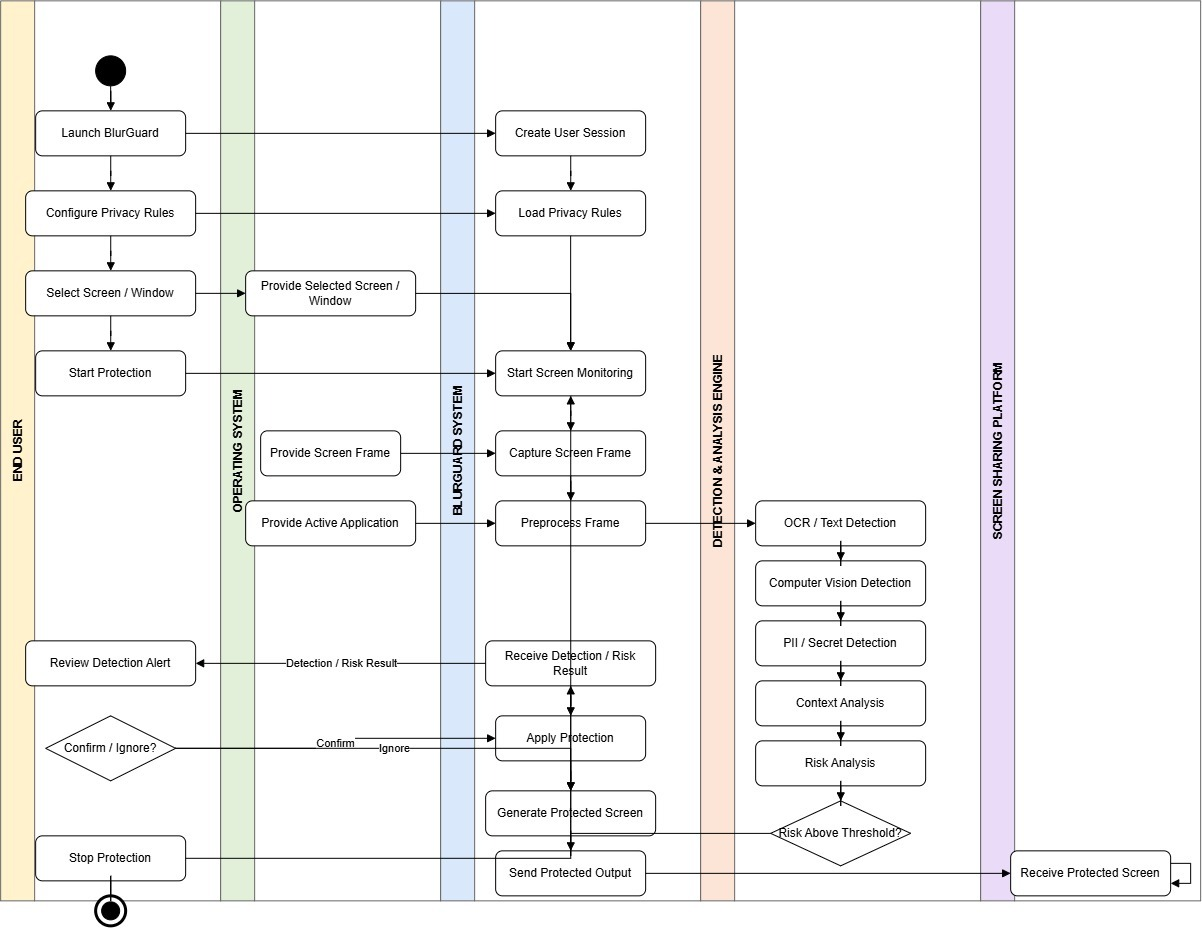
\includegraphics[width=\textwidth]{activity_swimlane_diagram.jpg}
\caption{Activity and Swimlane Diagram}
\end{figure}

\subsection{Sequence Diagram}

The sequence diagram shows the chronological interaction between the user interface and processing modules.

\begin{figure}[H]
\centering
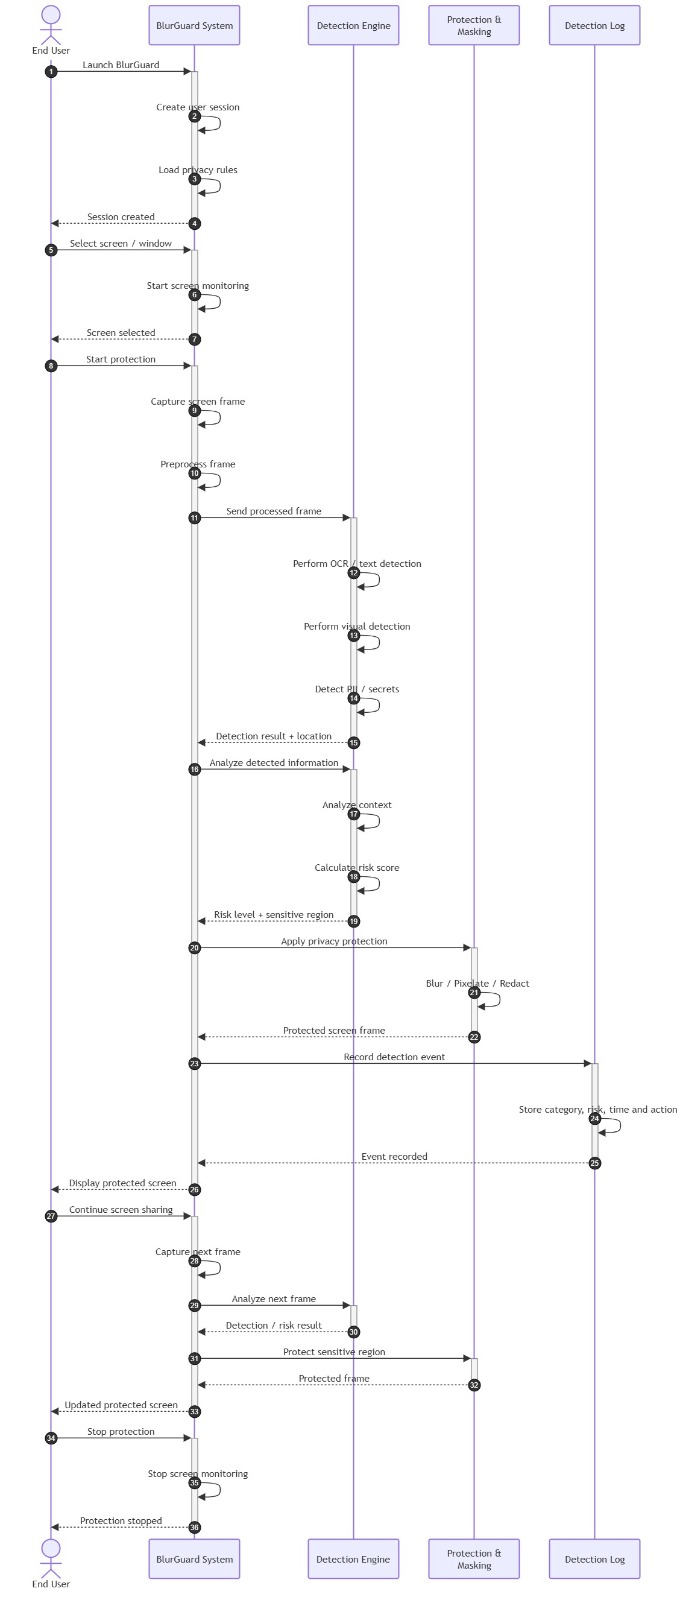
\includegraphics[width=0.72\textwidth]{sequence_diagram.jpg}
\caption{Sequence Diagram of BlurGuard}
\end{figure}

\subsection{Collaboration Diagram}

The collaboration diagram represents communication between the major BlurGuard components.

\begin{figure}[H]
\centering

\includegraphics[width=\textwidth]{collaboration_diagram.jpg}
\caption{Collaboration Diagram of BlurGuard}
\end{figure}

\subsection{Project Timeline}

The Gantt chart represents the planned development activities.

\begin{figure}[H]
\centering
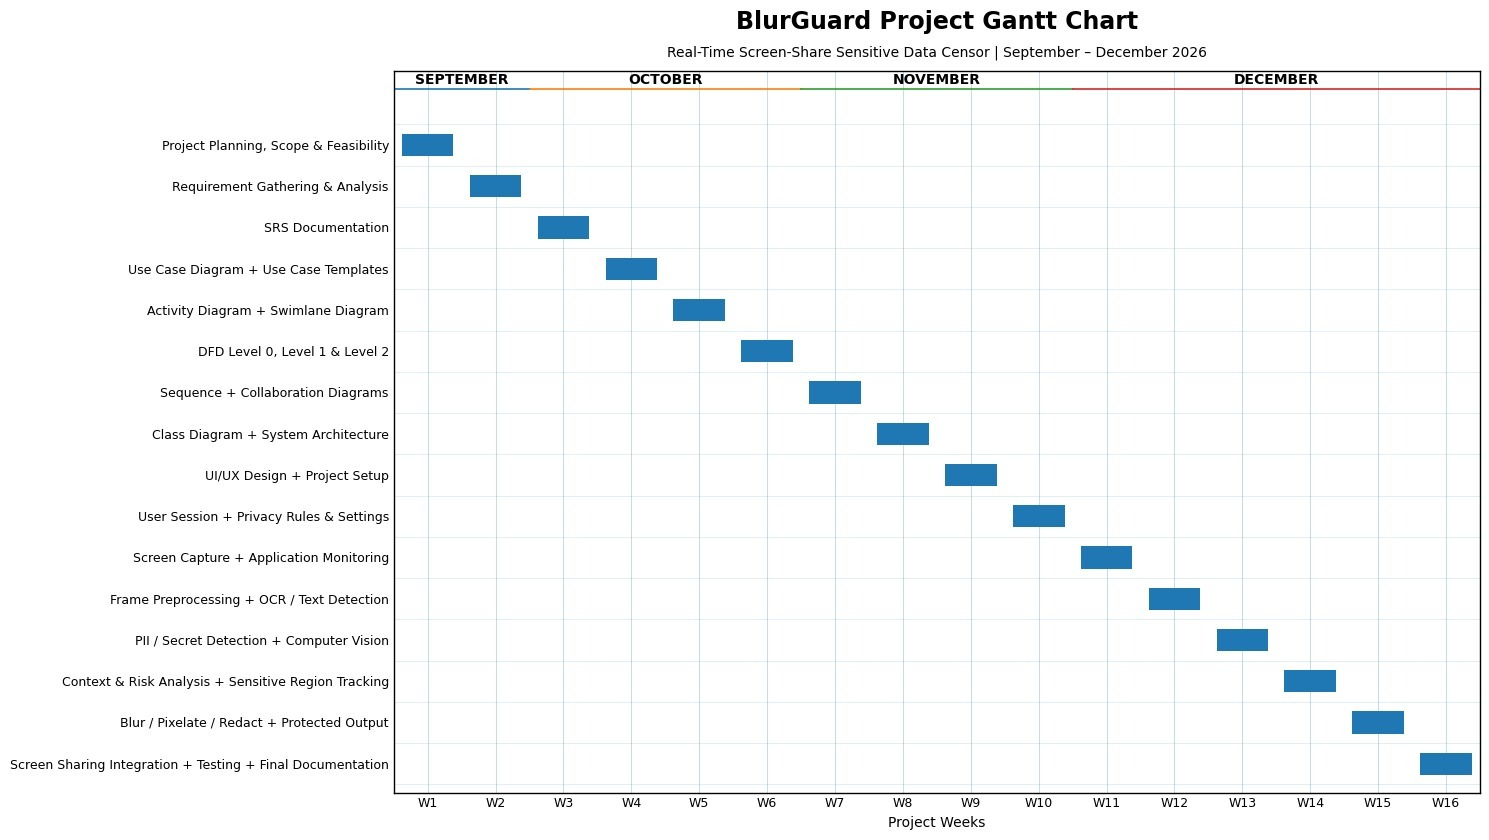
\includegraphics[width=\textwidth]{blurguard_gantt_chart.jpg}
\caption{Project Scheduling and Timeline}
\end{figure}

% =========================================================
% CHAPTER 3
% =========================================================

\chapter{Progress Evaluation}

\section{Current Status and Validation}

The project has completed the initial system architecture, interface design, UML modelling, and core privacy-protection workflow.

The current prototype includes:

\begin{itemize}
    \item Secure Workspace
    \item Privacy Command Center
    \item Live Monitoring interface
    \item Detection workflow
    \item Risk classification
    \item Masking approach
    \item UML system models
\end{itemize}

\section{Testing}

Testing will focus on:

\begin{itemize}
    \item OCR text extraction
    \item Sensitive-data detection
    \item Risk classification
    \item Region localisation
    \item Masking functionality
    \item Interface behaviour
\end{itemize}

The detection system can be evaluated using precision, recall, and F1-score after experimental testing.

\begin{equation}
Precision = \frac{TP}{TP+FP}
\end{equation}

\begin{equation}
Recall = \frac{TP}{TP+FN}
\end{equation}

\begin{equation}
F1 =
2\frac{Precision \times Recall}
{Precision + Recall}
\end{equation}

No numerical performance values are reported until actual experiments are completed.

% =========================================================
% CHAPTER 4
% =========================================================

\chapter{Conclusion}

\section{Summary of Work}

BlurGuard proposes an automated privacy-protection system for detecting and masking sensitive information in visual content.

The project combines image processing, OCR, pattern matching, risk assessment, and masking within a modular architecture.

The current work establishes the frontend interface, system workflow, UML models, and core detection approach.

\section{Future Work}

Future development will focus on:

\begin{itemize}
    \item Real-time screen capture
    \item Improved OCR
    \item Context-aware detection
    \item Named Entity Recognition
    \item Additional sensitive-data categories
    \item Screen-sharing integration
    \item Confidence-based masking
    \item Performance optimisation
\end{itemize}

% =========================================================
% BIBLIOGRAPHY
% =========================================================

\clearpage

\chapter*{Bibliography}
\addcontentsline{toc}{chapter}{Bibliography}

\begin{enumerate}

\item R. Smith, ``An Overview of the Tesseract OCR Engine,'' in
\textit{Proceedings of the Ninth International Conference on Document Analysis and Recognition}, 2007.

\item G. Bradski, ``The OpenCV Library,'' \textit{Dr. Dobb's Journal of Software Tools}, 2000.

\item S. Brin and L. Page, ``The Anatomy of a Large-Scale Hypertextual Web Search Engine,''
\textit{Computer Networks and ISDN Systems}, vol. 30, pp. 107--117, 1998.

\item OWASP Foundation, ``OWASP Application Security Verification Standard (ASVS),''
OWASP Foundation.

\item FastAPI Documentation, ``FastAPI: Modern Web Framework for Building APIs with Python.''

\item React Documentation, ``React: A JavaScript Library for Building User Interfaces.''

\end{enumerate}

% =========================================================

\end{document}